\section{Modelos usados}

En esta sección se explican los modelos que se han desarrollado. Se ha creado un modelo base y cuatro redes neuronales con cuatro arquitecturas distintas. Los resultados de estos modelos se pueden ver en la Sección \ref{results}.
\newline

\subsection{Modelo base}\label{baseline_model}
Antes de definir las redes neuronales de este trabajo, se ha realizado un estudio de otros trabajos y resultados similares que se puede observar en la sección \ref{similar_projects}. Esto permite poder usar los resultados de otros proyectos como punto de referencia, sabiendo si el desarrollo de esta práctica está mejorando los resultados obtenidos por otros proyectos o no. Además de tener los puntos de referencias de otros proyectos, se ha definido un modelo base.
\newline

Un modelo base es un modelo trivial que se suele desarrollar cuando se quiere resolver un problema de predicción o clasificación para saber si el resto de modelos que se van a desarrollar mejoraran el resultado. En este proyecto, el modelo base desarrollado no tiene lógica y simplemente devuelve el valor que hubo con una semana de anterioridad como predicción.  
\newline

A continuación se puede ver gráficamente las predicciones del modelo respecto a los valores reales:
\begin{figure}[H]
    \centering
    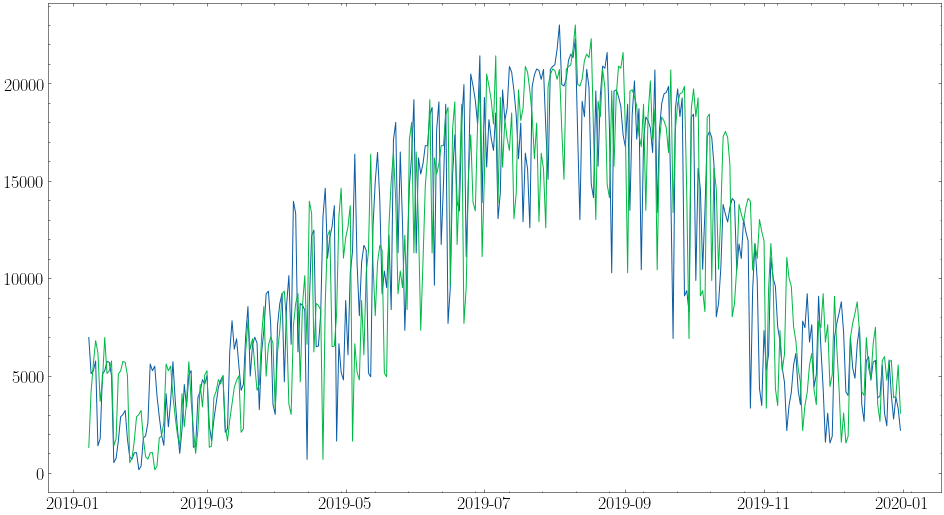
\includegraphics[width=16cm]{images/solution/predictions/baseline-predictions.png}
    \caption{Predicciones del modelo básico}
    \label{fig:baseline-predictions}
\end{figure}

Se puede observar que las predicciones son los mismo valores reales pero desplazados una semana. Una vez desarrollado este modelo, se han calculado las métricas que se muestran en la sección \ref{results} junto con el resto de los resultados de los otros modelos.

\subsection{Modelos con redes neuronales}
\subsubsection{Modelo denso}


Este modelo es un modelo con solo capas de tipo \textit{forward-pass}. Tiene otras dos capas pero que no implementan lógica asociada a lo que es la red neuronal en sí, sino que son capas de traducción de matriz a vector y viceversa como se explicará a continuación. Gráficamente la red que se ha definido es la siguiente:
\begin{figure}[H]
    \centering
    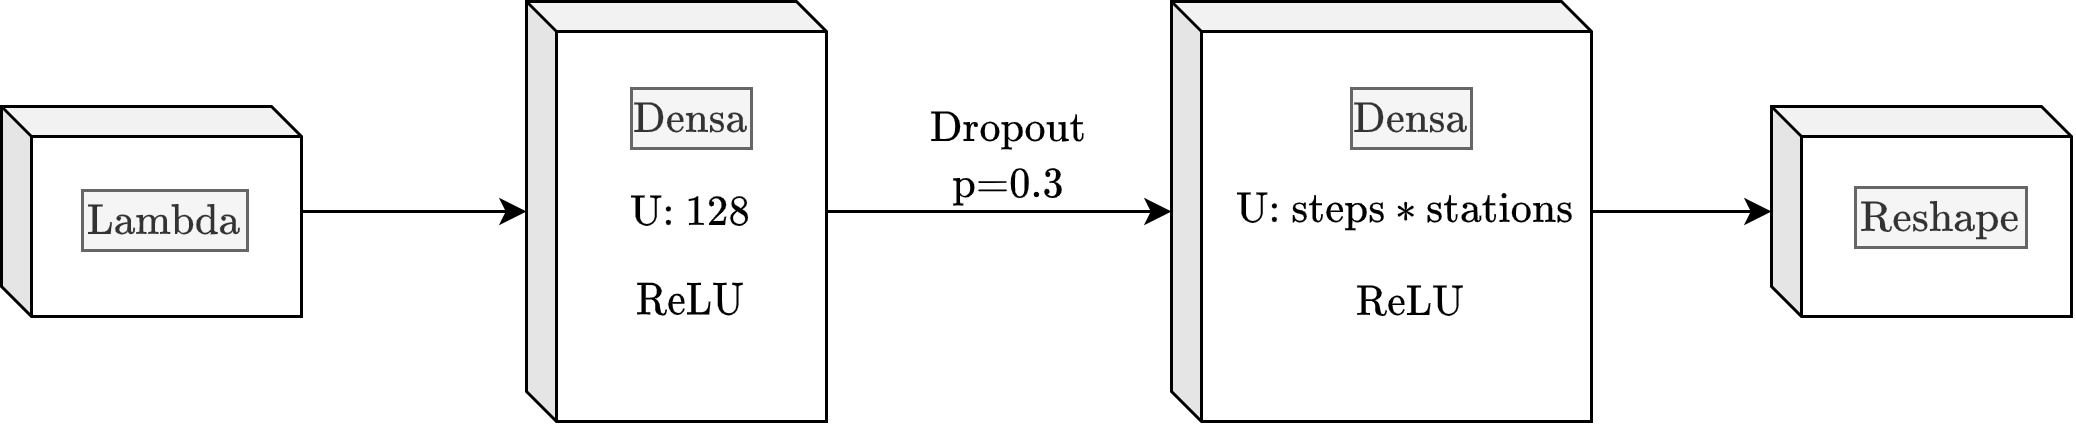
\includegraphics[width=12cm]{images/solution/models/dense.png}
    \caption{Modelo denso}
    \label{fig:dense-model}
\end{figure}

La primera capa oculta tiene 128 unidades. La cantidad de neuronas que tiene una capa oculta es un parámetro que se ha puesto de forma pseudoaleatoria. Se han realizado distintas combinaciones probando distintas cantidades de unidades y 128 es el que mejor resultado a dado. La segunda capa oculta tiene la misma cantidad de unidades que valores tiene que devolver el modelo, que es un valor calculado por la multiplicación entre el número de estaciones con las que se está trabajando, 633, por el número de intervalos que se quieren calcular. Por ejemplo, si se quiere calcular un único intervalo para todas las estaciones, el vector de dicha capa será de $633$ elementos, si se quiere calcular dos intervalos, el número de elementos del vector será $1266 = 2 \times 633$ y así sucesivamente. Esta capa es común a todos los modelos que se explicarán de aquí en adelante.
\newline

La última capa es una capa de tipo \textit{Reshape}. Esta capa no tiene ni función de activación ni parámetros que ajustar porque lo único que hace es ajustar el vector de la capa anterior a una matriz más comprensible y con la que se puede trabajar de forma más cómoda con el dataset. Básicamente, devolverá un vector de vectores, donde cada elemento será un intervalo y cada intervalo tendrá la predicción para cada estación. Siguiendo la misma lógica, la primera capa es de tipo \textit{Lambda} y se encarga de realizar la tarea opuesta, dada una matriz obtener un vector. Las capas \textit{Lambda} son capas en las que el usuario define una función que se quiera ejecutar.
\newline

El código de este modelo se ha definido como se muestra a continuación:

\begin{minted}[fontsize=\scriptsize]{python}
from tensorflow.keras.models import Sequential
from tensorflow.keras.layers import Reshape, Dense, Dropout, Lambda

# `steps` is a variable which has the number of intervals to be predict
steps = 0 

# `stations` is the number of stations in the bike network
stations = 0

dense_model = Sequential([
    # Matrix to vector
    Lambda(lambda x: x[:, -1:, :]), 
    
    # Input layer
    Dense(128, activation="relu"),

    Dropout(0.3),
    
    # Ouput layer
    Dense(steps * stations),
                  
    # Vector to matrix
    Reshape([steps, stations])
])
\end{minted}


Los resultados del modelo se pueden ver junto al resto de resultados en la sección \ref{results}.
\subsubsection{Modelo recurrente básico}

Este modelo es el mismo modelo que el denso pero añadiendo una nueva capa recurrente simple explicada en la sección \ref{rnn_theory}. La capa recurrente simple es una capa que nos permite usar información de otros intervalos anteriores que serán usados para la predicción final. Esta capa recurrente tiene 100 unidades y gráficamente el modelo se puede representar de la siguiente forma:
\begin{figure}[H]
    \centering
    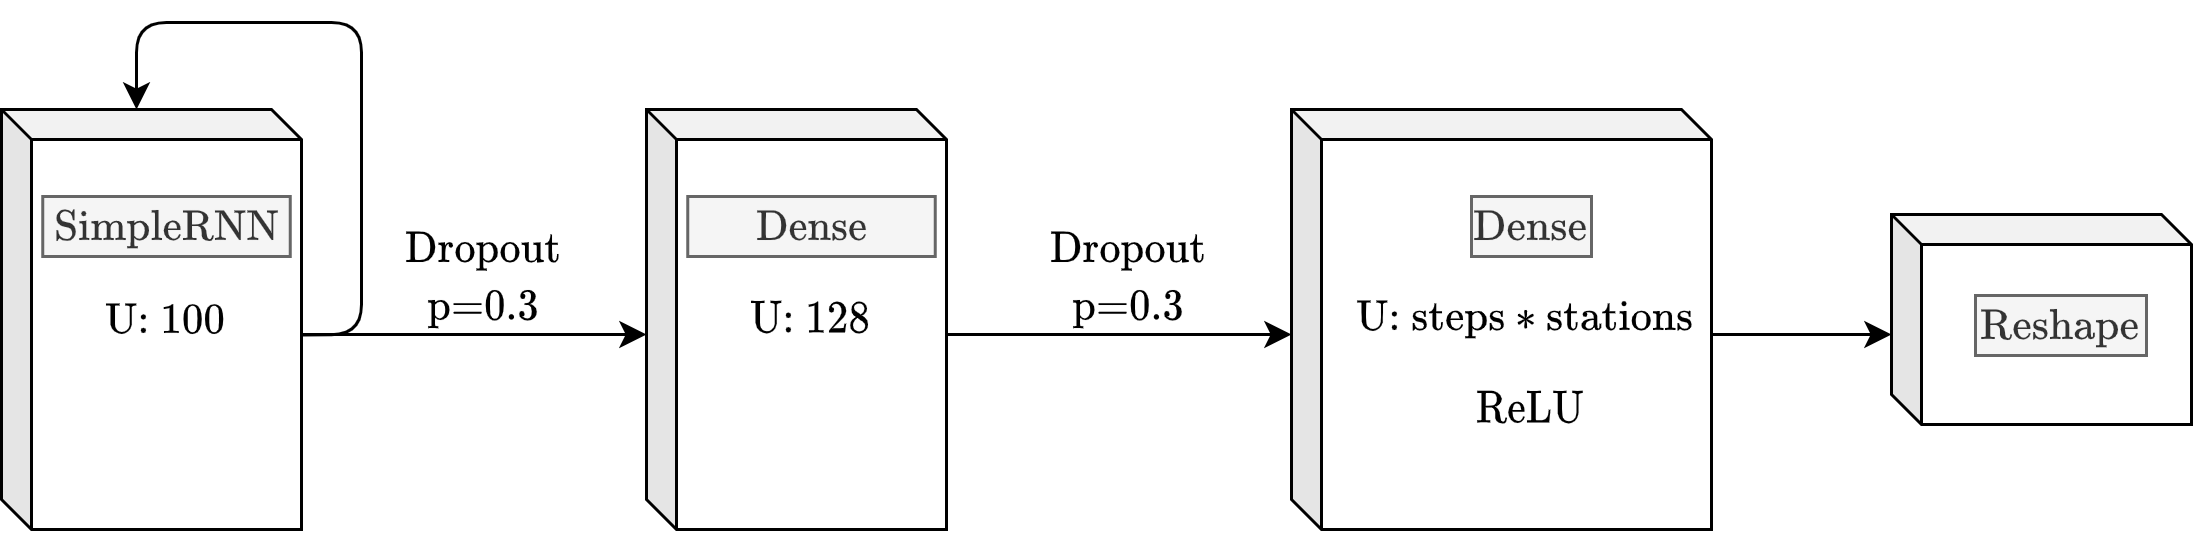
\includegraphics[width=12cm]{images/solution/models/simpleRnn.png}
    \caption{Modelo recurrente básico}
    \label{fig:dense-model}
\end{figure}

Como se puede observar es una extensión del modelo denso explicado en la sección anterior pero añadiendo una nueva capa de tipo \textit{SimpleRNN}. El código de este modelo se ha definido como se muestra a continuación:
\begin{minted}[fontsize=\scriptsize]{python}
from tensorflow.keras.models import Sequential
from tensorflow.keras.layers import Reshape, Dense, Dropout, Lambda, SimpleRNN

# `steps` is a variable which has the number of intervals to be predict
steps = 0 

# `stations` is the number of stations in the bike network
stations = 0

rnn_model = Sequential([
    # Matrix to vector
    Lambda(lambda x: x[:, -1:, :]),
    
    SimpleRNN(100, return_sequences=True),
    
    Dropout(0.3),
    Dense(128),
    Dropout(0.3),
    
    # Ouput layer
    Dense(steps * stations),
    
    # Vector to matrix
    Reshape([steps, stations])
])
\end{minted}


Los resultados del modelo se pueden ver junto al resto de resultados en la sección \ref{results}.
\subsubsection{Modelo recurrente LSTM}

Este modelo es igual que el modelo recurrente básico pero sustituyendo la capa recurrente por una capa LSTM la cual es más compleja y permite que la red aprenda más patrones que están distribuidos en el tiempo como se explicó en la sección \ref{lstm_theory}. Esta capa recurrente tiene 128 unidades y gráficamente el modelo se puede representar de la siguiente forma:
\begin{figure}[H]
    \centering
    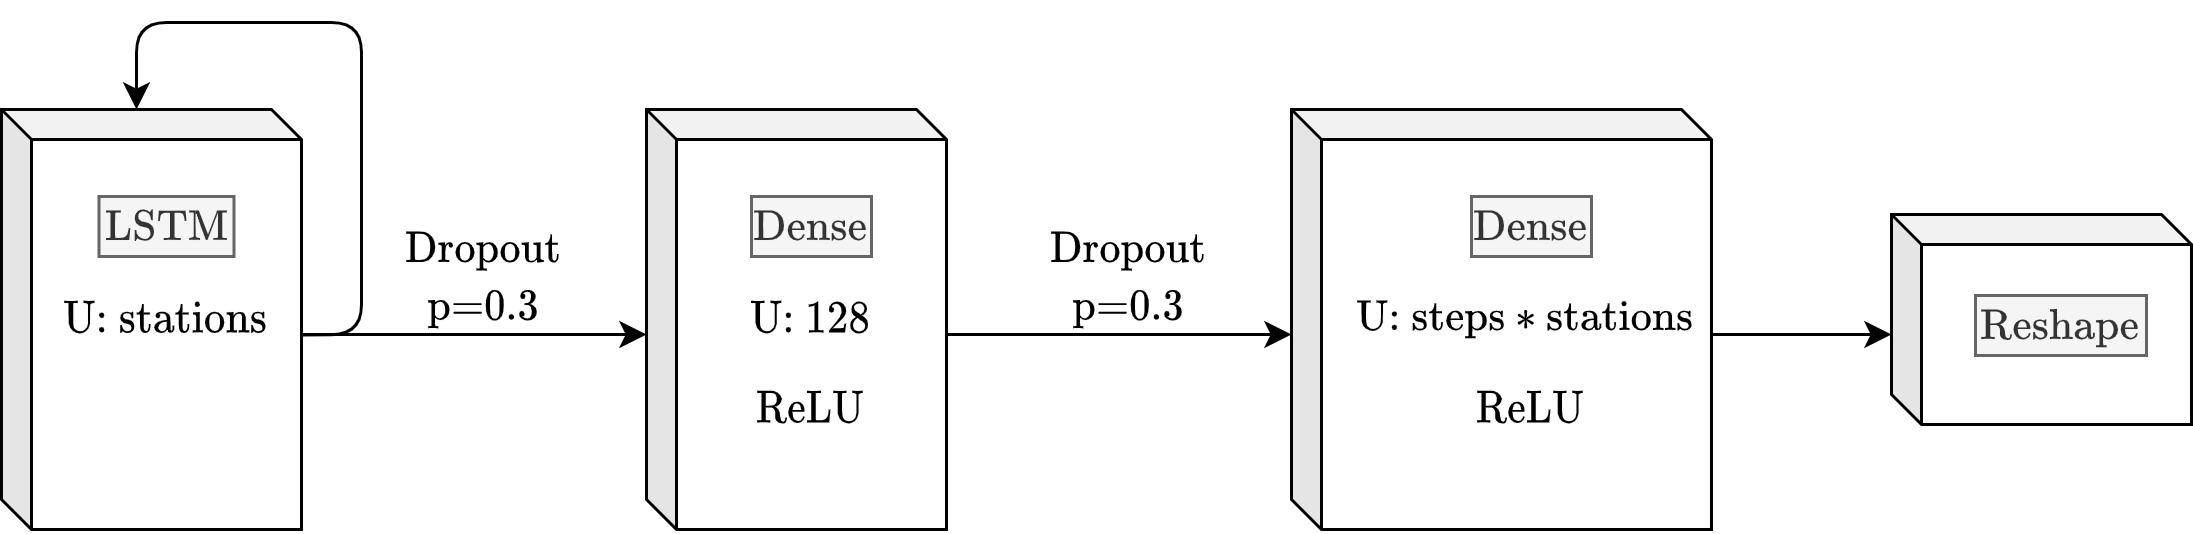
\includegraphics[width=12cm]{images/solution/models/LSTM.png}
    \caption{Modelo recurrente LSTM}
    \label{fig:dense-model}
\end{figure}

Como se puede observar es el mismo modelo pero sustituyendo la capa \textit{SimpleRNN} por una \textit{LSTM}. El código de este modelo se ha definido como se muestra a continuación:
\begin{minted}[fontsize=\scriptsize]{python}
from tensorflow.keras.models import Sequential
from tensorflow.keras.layers import Reshape, Dense, Dropout, Lambda, LSTM

# `steps` is a variable which has the number of intervals to be predict
steps = 0 

# `stations` is the number of stations in the bike network
stations = 0

lstm_model = Sequential([
    # LSTM layer
    LSTM(stations, return_sequences=False),
    
    Dropout(0.3),
    Dense(128, activation="relu"),
    
    # Output layer
    Dropout(0.3),
    Dense(steps * stations, activation="relu"),
    
    # Vector to matrix
    Reshape([steps, stations])
])
\end{minted}

Los resultados del modelo se pueden ver junto al resto de resultados en la sección \ref{results}.
\subsubsection{Modelo autoregresivo (AR)}\label{model_ar}


Un modelo autoregresivo es otro tipo de redes neuronal recurrente. Esta red tiene como peculiaridad que el resultado obtenido se usa como valor de entrada para el calculo de la siguiente iteración. El modelo generado gráficamente es el siguiente:
\begin{figure}[H]
    \centering
    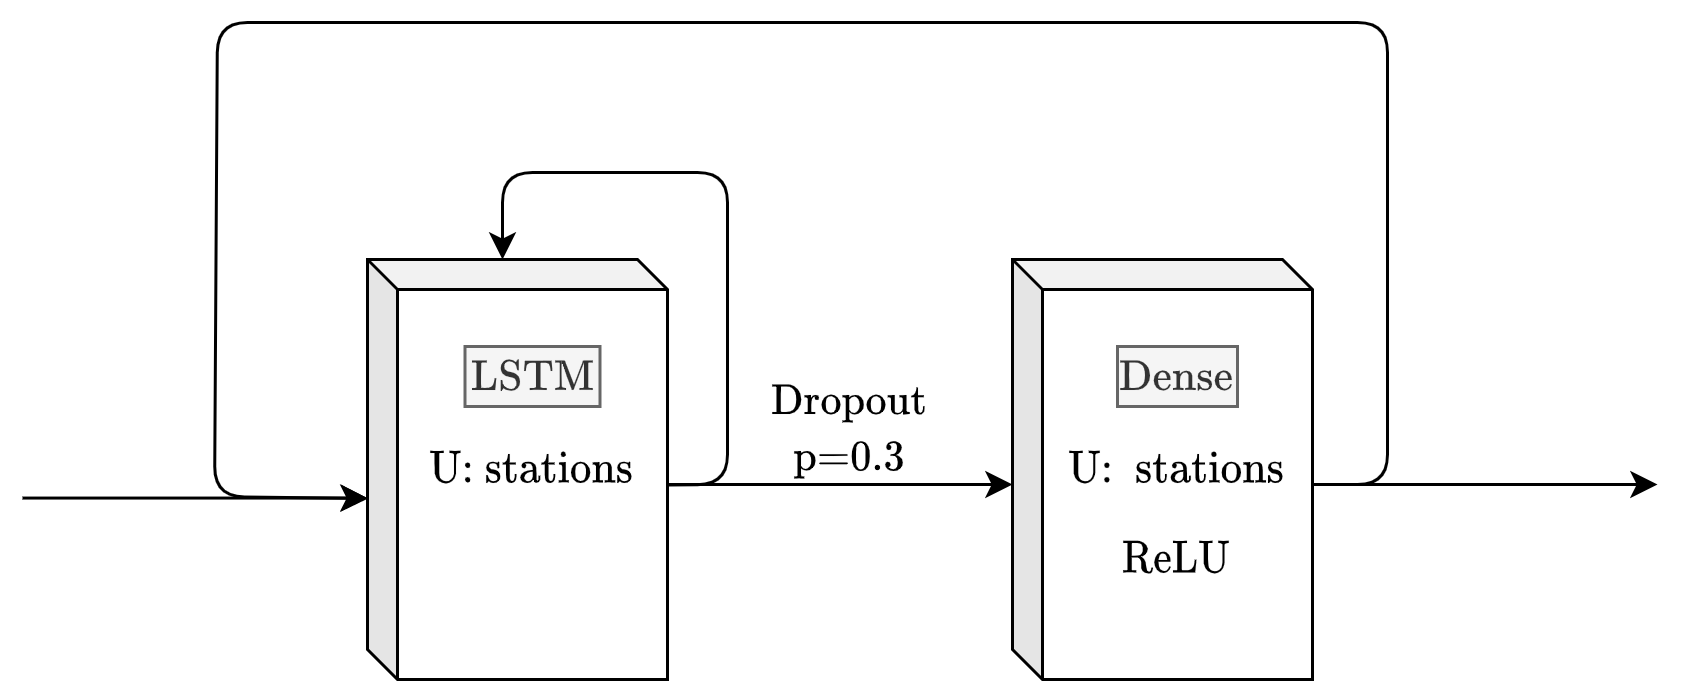
\includegraphics[width=10cm]{images/solution/models/AR.png}
    \caption{Modelo recurrente Autoregresivo}
    \label{fig:dense-model}
\end{figure}

El modelo tiene una capa LSTM junto con una capa densa. La salida de esta capa que es la predicción del modelo se reintroduce en el modelo para predecir el resto de predicciones.
\newline

\textit{Tensorflow} no dispone de un modelo en su librería que supliese las necesidades que buscábamos, por esa razón, se ha tenido que implementar este modelo usando otra técnica. Se ha creado una clase nueva que hereda de \small\verb|tf.keras.Model| y la cual tiene tres métodos: \small\verb|__init__|, \small\verb|warmup| y \small\verb|call|. De esta forma se pueden generar modelos que puedan tener arquitecturas singulares y distintas a las \textit{pass-forward}. Para la implementación se ha seguido la documentación de \textit{Tensorflow} \cite{tensorflow2015-whitepaper} y \textit{Keras} \cite{keras}.
\newline

La clase usada para definir el modelo autoregresivo ha sido el siguiente:
\begin{minted}[fontsize=\scriptsize]{python}
import tensorflow as tf
from tensorflow.keras.layers import LSTMCell, RNN, Dense

class AutoRegressive(tf.keras.Model):
    def __init__(self, lstm_units, steps, stations):
        super().__init__()
        self.steps = steps
        self.stations = stations
        self.lstm_units = lstm_units
        
        # First LSTM layer
        self.lstm_cell = LSTMCell(lstm_units)
        # Also wrap the LSTMCell in an RNN to simplify the `warmup` method.
        self.lstm_rnn = RNN(self.lstm_cell, return_state=True)
        
        # Ouput layer
        self.dense = Dense(stations, activation="relu")

    def warmup(self, inputs):
        # inputs.shape => (batch, time, features)
        # x.shape => (batch, lstm_units)
        x, *state = self.lstm_rnn(inputs)

        # predictions.shape => (batch, features)
        prediction = self.dense(x)
        return prediction, state

    def call(self, inputs, training=None):
        # Use a TensorArray to capture dynamically unrolled outputs.
        predictions = []

        # Initialize the lstm state
        prediction, state = self.warmup(inputs)

        # Insert the first prediction
        predictions.append(prediction)

        # Run the rest of the prediction steps
        for n in range(1, self.steps):
            # Use the last prediction as input.
            x = prediction
            
            # Concat with timestamp variables
            x = tf.concat([x, inputs[:,-1,-3:]], 1)
            
            # Execute one lstm step.
            x, state = self.lstm_cell(x, states=state, training=training)
                                      
            # Convert the lstm output to a prediction.
            prediction = self.dense(x)
            
            # Add the prediction to the output
            predictions.append(prediction)

        # predictions.shape => (time, batch, features)
        predictions = tf.stack(predictions)
        
        # predictions.shape => (batch, time, features)
        predictions = tf.transpose(predictions, [1, 0, 2])
        
        return predictions
\end{minted}


Para crear un nuevo modelo simplemente se genera una nueva instancia de la siguiente manera:
\begin{minted}[fontsize=\scriptsize]{python}
AutoRegressive(lstm_units=stations, steps=steps, stations=stations)
\end{minted}

Los resultados del modelo se pueden ver junto al resto de resultados en la sección \ref{results}.
\subsection{Ventanas}

Como se ha explicado en la sección \ref{window-generator}, se pueden generar predicciones en función de los argumentos de entrada. Es decir, se puede crear un modelo que dado una cantidad $X$ de intervalos, pueda predecir una cantidad $Y$ de intervalos. Se quería comparar diferentes ajustes que se pueden realizar a las ventanas y ver los resultados obtenidos. En definitiva, se ha creado un modelo distinto para cada uno de los tamaños de ventana.
\newline

De aquí en adelante, se hará referencia a las configuración de ventana con tuplas, donde el primer término es el tamaño de intervalos de entrada y el segundo elemento el tamaño de intervalos que el modelo predice. Por ejemplo dada la siguiente tupla 12-5, quiere decir que el modelo desarrollado usa una ventana con 12 intervalos de entrada y 5 intervalos de salida.
\newline

En total se han usado 15 configuraciones de ventana distintas: 3-1, 5-1, 8-1, 8-3, 8-5, 12-1, 12-3, 12-5, 24-1, 24-3, 24-5, 36-8, 36-12, 48-12, 48-24. Como se han desarrollado 4 arquitecturas de neuronales diferentes, al final se han desarrollado 60 modelos más el modelo básico. 

\subsection{Entrenamiento, validación y test de las redes neuronales}


Una vez creado los modelos, se ha codificado una función para automatizar el proceso de entrenamiento, validación y test de cada uno de los modelos y de además de obtener las métricas que se necesitarán para poder estudiar y comparar los distintos modelos. El código es el siguiente:

\begin{minted}[fontsize=\scriptsize]{python}

MAX_EPOCHS = 150

'''
Compiles and train model

@param model which will be training
@param window with the Datasets used
@param max_epoch for training
@param should_stop if detects overfitting the stops with a patience of 10
@param lr (learning rate) of the model
'''
def compile_and_fit(model, window, max_epochs=MAX_EPOCHS, should_stop=False, lr=0.001):
    model.compile(
        loss=tf.losses.Huber(),
        optimizer=tf.optimizers.Adam(lr=lr),
        metrics=[MeanSquaredLogarithmicError(), MeanSquaredError(), MeanAbsoluteError(),
                RootMeanSquaredError(), RootMeanSquaredLogarithmicError])
    
    # Define the callbacks for the training proccess
    # PlotLossesKeras plots training and validation for every epoch in real time
    # early_stopping allows to stop if detects overfitting
    cbs = [PlotLossesKeras()] + ([EarlyStopping(monitor='val_loss',
                                                      patience=10,
                                                      mode='min')] if should_stop else [])
    
    model.fit(window.train, epochs=max_epochs,
                        validation_data=window.val,
                        callbacks=cbs,
                        verbose=2)
    
'''
Computes metrics and returns it as DataFrame
'''
def get_metrics(model, window):
    train_metrics = model.evaluate(window.train)
    val_metrics = model.evaluate(window.val)
    test_metrics = model.evaluate(window.test)

    metrics_names = model.metrics_names
    metrics_names[0] = "huber"
    metrics = pd.DataFrame({
        "names": metrics_names,
        "train": train_metrics,
        "val": val_metrics,
        "test": test_metrics,
    })

    return metrics


windows_sizes=[(3, 1), (5, 1), (8, 1), (8, 3), (8, 5), (12, 1), 
                (12, 3), (12, 5), (24, 1), (24, 3), (24, 5)]

'''
Given a model it will train with different windows sizes

@param model which will be training
@param max_epoch for training
@param lr (learning rate) of the model
@param windows_sizes a list of tuples containing window sizes as (input, output)
'''
def model_generator(model, lr, max_epochs=150, windows_sizes=windows_sizes):
    # Loads and splits the DataFrames
    df = load_dataset()
    train_df, val_df, test_df = split_dataset(df)
    
    # For every windo
    for w in windows_sizes:
        # Create the windoe
        input_width, steps = r
        window = WindowGenerator(input_width=input_width,
                                 label_width=steps,
                                 shift=steps,
                                 train_df=train_df,
                                 val_df=val_df,
                                 test_df=test_df)

        
        # Train model
        compile_and_fit(
            model, window, lr=lr, should_stop=True, max_epochs=max_epochs)
        
        # Save metrics
        metrics = get_metrics(model, window)
        filename = "/path/to/results/{model.get_name()}" + \
                    "-{input_width}-{steps}.csv"
        metrics.to_csv(filename)
\end{minted}


Como se puede ver en el código, dado un modelo, la función se encarga de entrenar dicho modelo pero con distintas configuraciones de ventana y posteriormente guarda las métricas en un CSV. 